\documentclass[conference]{IEEEtran}




% correct bad hyphenation here
\hyphenation{op-tical net-works semi-conduc-tor}
\usepackage{graphicx}
\usepackage{pifont}% http://ctan.org/pkg/pifont
\usepackage{url}
\usepackage{enumitem}
\usepackage{algorithm}
\usepackage{algpseudocode}
\usepackage{pifont}
% Allow commas and periods to extend into margin slightly.
\usepackage[protrusion=true,expansion=true]{microtype}
\newcommand{\cmark}{\ding{51}}%
\newcommand{\xmark}{\ding{55}}%
\newcommand\floor[1]{\lfloor#1\rfloor}

\begin{document}
\title{Quantifying Semantic Similarity of Software Projects Using Deep Semantic Similarity Model(DSSM)}




%%%%%%%% Other format %%%%%%%%%%%%%
\author{
    Akond Ashfaque Ur Rahman\\
    Department of Computer Science\\
    North Carolina State University\\
    Raleigh, North Carolina, USA\\
    aarahman@ncsu.edu 

}
%%%%%%%%%%%%%%%%%%%%%%%%%%%%%%%%%%%%


% make the title area
\maketitle

% As a general rule, do not put math, special symbols or citations
% in the abstract
\begin{abstract}


Software re-usability can help software organizations to achieve rapid construction of software saving software teams in effort and time. Finding similar projects within a software organization as well as within the open source domain, can help software teams to gather source code that can be re-usable helping them to construct software at a faster rate. \textit{The goal of this paper is to help software teams in facilitating software re-usability using semantic similarity and deep learning techniques on source code of software applications.} The author uses available open source techniques to gather natural language tokens from software projects, and use them with deep learning techniques to quantify semantic similarity. The author uses Microsoft's Deep Semantic Similarity Model (DSSM) to quantify semantic similarity on nine open source software projects. The paper also includes relevant empirical findings that illustrates how the proposed methodology works with nine real-world software projects obtained from Github. In addition to the empirical findings, the author discusses how the proposed methodology can be extended to advance industry and academic research in the area of software reuse and increased productivity.   


\end{abstract}


\IEEEpeerreviewmaketitle

\begin{IEEEkeywords} 

software repositories; semantic similarity; Deep Semantic Similarity Model (DSSM)

\end{IEEEkeywords}



%%%%%%%%%%%%%%%%%%%%%%%%%%%%%%%%%%%%%%%%%%%%%%%%%%%%%%%%%%%%%
%%%%%%%%%%%%%%%%%%%%% This is introduction section %%%%%%%%%%
%%%%%%%%%%%%%%%%%%%%%%%%%%%%%%%%%%%%%%%%%%%%%%%%%%%%%%%%%%%%%

\section{Introduction}


Lim~\cite{Lim:Reuse:Quality} observed that re-use of software components overall has a positive impact on software quality. Lim observed that when software is re-used in a software team, defects decreases, and productivity increases. Software teams can use different aspects of software artifacts to achieve software re-usability e.g., architecture of the software, source code and of the software, and designs and documentations of the software~\cite{Reuse:Aspects:Frakes}. Amongst these numerous aspects of software artifacts, source code of software is the most frequently referred artifacts for software reuse~\cite{Google:SoftwareReuse}. Researcher has observed that software engineers tend to adopt different strategies to identify and manipulate re-usable portions of software code such as syntax-based search using \textit{grep-like} tools, communicating with colleagues, and using the web~\cite{Google:SoftwareReuse}. These strategies can be time and effort consuming leading to reduced productivity~\cite{zimmerman:code:search}. Automated tools that quantifies similarity amongst software projects can help software developers to identify and work on re-usable portions of existing software codebase. This paper proposes and illustrates a methodology that quantifies the semantic similarities between software projects in order to help software developers in finding similar software projects and software components.
%%Grechanik et al.`\cite{Grechanik:Exemplar} provided empirical evidence on how semantic-based search tools can help software developers to find similar applications.                 
\textit{The goal of this paper is to help software teams in facilitating software re-usability using semantic similarity and deep learning techniques on source code of software applications.}
The author proposes a methodology that parses codebases of software repositories to create a list of natural language tokens, and use that collection of natural language tokens to investigate the semantic similarity between software projects. The author has used open source utilities such as SrcML.NET\footnote{https://github.com/abb-iss/SrcML.NET}, and Swum.NET\footnote{https://github.com/abb-iss/Swum.NET} to parse and filter the software projects into natural language tokens. The author has also used Microsoft's \textit{Deep Semantic Similarity Model (DSSM)} and \textit{Sent2Vec}\footnote{http://research.microsoft.com/en-us/projects/dssm/} utilities to investigate and quantify the semantic similarity between different software projects. The author chose open source software projects written in C, C\#, and Java from Github\footnote{http://github.com/} to illustrate how the proposed methodology works. In this work the author has also presented if different combinations of DSSM parameters can impact the semantic similarity between software projects. 
The author presents the contributions of this paper as following: 
\begin{itemize}
\item{A proposed methodology that illustrates how Microsoft's DSSM and Sent2Vec utilities can be used to quantify the semantic similarity between software projects.}
\item{A discussion on how the proposed methodology can be used to advance industry and academic research in the domain of software re-usability.}
\end{itemize}    

The rest of the paper is organized as follows: the author provides background information and related work in Section~\ref{related}. The author presents the methodology in Section~\ref{meth}. The author presents empirical findings in Section~\ref{results}. The author discuss the findings of the study in Section~\ref{discussion}. The limitations of the study are presented in Section~\ref{limitation}. Challenges in conducting the study is presented in Section~\ref{challenges}. Finally the author concludes the paper in Section~\ref{conclusion}.




%%%%%%%%%%%%%%%%%%%%%%%%%%%%%%%%%%%%%%%%%%%%%%%%%%%%%%%%%%%%%
%%%%%%%%%%%%%%%%%%%%% This is background section %%%%%%%%%%%%
%%%%%%%%%%%%%%%%%%%%%%%%%%%%%%%%%%%%%%%%%%%%%%%%%%%%%%%%%%%%%


\section{Background and Related Work}
\label{related}
The author uses this section to describe the necessary concepts used in the study as well as prior academic studies that are related to this paper.
\subsection{Background}
The author provides brief background on the utilities that have been used in the paper. 
\subsubsection{SrcML.NET}
SrcML.NET is a framework developed in C\# that is used to perform program transformation and code analysis. SrcML.NET is based on the `srcML' project from Kent State University Software Development Laboratory. SrcML.NET provides an API to extract source code elements from a software project. In this study the author extracted raw natural language tokens from software projects and stored them in XML formats. The granularity of extracting the natural language tokens is at a file level i.e. in the XML file the corresponding tokens of one file was indexed according to its file name.    
\subsubsection{Swum.NET}
Swum.NET is a tool developed in C\# that removes alpha-numeric symbols 
and converts identifiers constructed in a camel case or pascal case format to get the natural language tokens.    
\subsubsection{Deep Semantic Similarity Model (DSSM)}
DSSM is a variant of deep neural networks designed for text analysis. DSSM can be trained on large collection of text documents, and maps source-target document pairs to feature vectors in a latent space in such a way that the distance between source documents and their corresponding target documents in that space is minimized. In this paper, natural language tokens extracted from software projects are used as source and target document pairs. Gao et al.~\cite{gao:interesting:emnlp} demonstrated the effectiveness of DSSM using two tasks that reveal interestingness namely, automatic highlighting and contextual entity search. 
DSSM has different parameters that can be tuned to setup different experiments for the purpose of study. The author has used different values for the \textit{MAX\_ITER} parameter in this paper. MAX\_ITER corresponds to the maximum number of iterations to train DSSM.   

\subsubsection{Sent2Vec}
Sent2Vec is a utility that maps a pair of short natural language tokens to a pair of feature vectors in a continuous, low-dimensional space where the semantic similarity between the natural language tokens is computed as the cosine similarity between their vectors in that space. Sent2Vec performs the mapping using the DSSM. 
Sent2Vec has different parameters that can be tuned to setup different experiments. The parameters that have been used in the study are: 
\begin{itemize}
\item{\textit{inSrcModel} : the neural network to embed the source string.}
\item{\textit{inTgtModel} : the neural network to embed the target string.}
\item{\textit{inFilename} : the input sentence pair file where each line is a pair of natural language tokens, separated by tab. For this paper the set of natural language tokens presented before the tab comes from one of the two software projects that are being compared. The natural language tokens of the other software project are added after the tab.   }
\item{\textit{inSrcModelType} : the type of the source model, which can be DSSM or CDSSM. In this paper for all the experiments the author uses DSSM.}
\item{\textit{inTgtModelType} : the type of the source model, which can be DSSM or CDSSM. In this paper for all the experiments the author uses DSSM.}
\item{\textit{outFilenamePrefix} : the filename prefix to be used to output the similarity scores and the semantic vectors of the natural language tokens that are served as input.}
\end{itemize}


\subsection{Semantic Similarity in Software Engineering}
%Merkl et al.~\cite{merkl:similarity:related} used artificial neural networks to find similar features between software projects.
%Grechanik et al.~\cite{Grechanik:Exemplar} proposed and evaluated \textit{Exemplar}, and provided empirical findings showing how semantic-based techniques can help to identify relevant applications for software developers.
%Kawaguchi et al.~\cite{Kawaguchi:oss:cluster:related} proposed and introduced \textit{MUDABlue} that uses semantic information of open source projects to categorize open source projects without prior information.
%Marcus et al.~\cite{marcus:clone:related} used latent semantic indexing to determine conceptually similar software components such as functions, files, and code segments that are duplicated across the software.

%Srinivas et al.~\cite{Srinivas:similarity:related} used distribution of features through semantic similarity to cluster and classify software projects. Kuhn et al.~\cite{Kuhn:simialrity:related} used Latent Semantic Indexing (LSI) to group components of the software that are semantically similar.

%In another work Kuhn et al.~\cite{kuhn:sim:re:related} used semantic similarity to enrich the reverse engineering steps of software projects.

%Asuncion et al.~\cite{asuncion:sim:trace:related} used semantic similarity to facilitate software traceability in large scale software projects.

The paper is closely related to prior academic works that have investigated on how semantic similarity can be used to aid software developers and software teams. Cubranic et al.~\cite{Cubranic:hipikat:related} created and proposed a tool called \textit{Hipikat} that used semantic features of software tasks to recommend next probable software modification tasks within an IDE. Maletic et al.~\cite{Maletic:simila:rel} investigated and provided empirical findings on how semantic and structural information of source code elements can facilitate software developers in understanding software programs. Kiefer et al.~\cite{Kiefer:ontlogy:rel} investigated how semantic features of software repositories extracted using Web Ontology Languages can be used to characterize a software's evolution. Jalbert et al.~\cite{jalbert:bug:related} leveraged on textual semantics of bug reports to identify duplicate bugs in order to reduce development cost. Antoniol et al.~\cite{antoniol:link:related} used information retrieval to investigate how connections between the source code and documentation can be discovered. Yao et al.~\cite{Yao:reuse:related} used a semantic-based approach to classify and extract necessary information from re-usable software components.        
    
This paper takes a different stance on how semantic features of software projects can be beneficial for software teams and software developers. This paper proposes a methodology that takes natural language tokens as input to DSSM, and uses the trained DSSM to quantify the semantic similarity amongst multiple software projects.                



%%%%%%%%%%%%%%%%%%%%%%%%%%%%%%%%%%%%%%%%%%%%%%%%%%%%%%%%%%%%%
%%%%%%%%%%%%%%%%%%%%% This is methodology section %%%%%%%%%%%%
%%%%%%%%%%%%%%%%%%%%%%%%%%%%%%%%%%%%%%%%%%%%%%%%%%%%%%%%%%%%%


\section{Methodology}
\label{meth}
The author uses this section to describe the steps to perform relevant implementation and analysis. As shown in Figure~\ref{fig-meth}, the study involved four major steps namely, collection of software repositories, extracting tokens, training models, and obtaining similarity scores. Finally the author ends this section by describing the experiments used in this study.    
\begin{figure}[htbp]
\centering
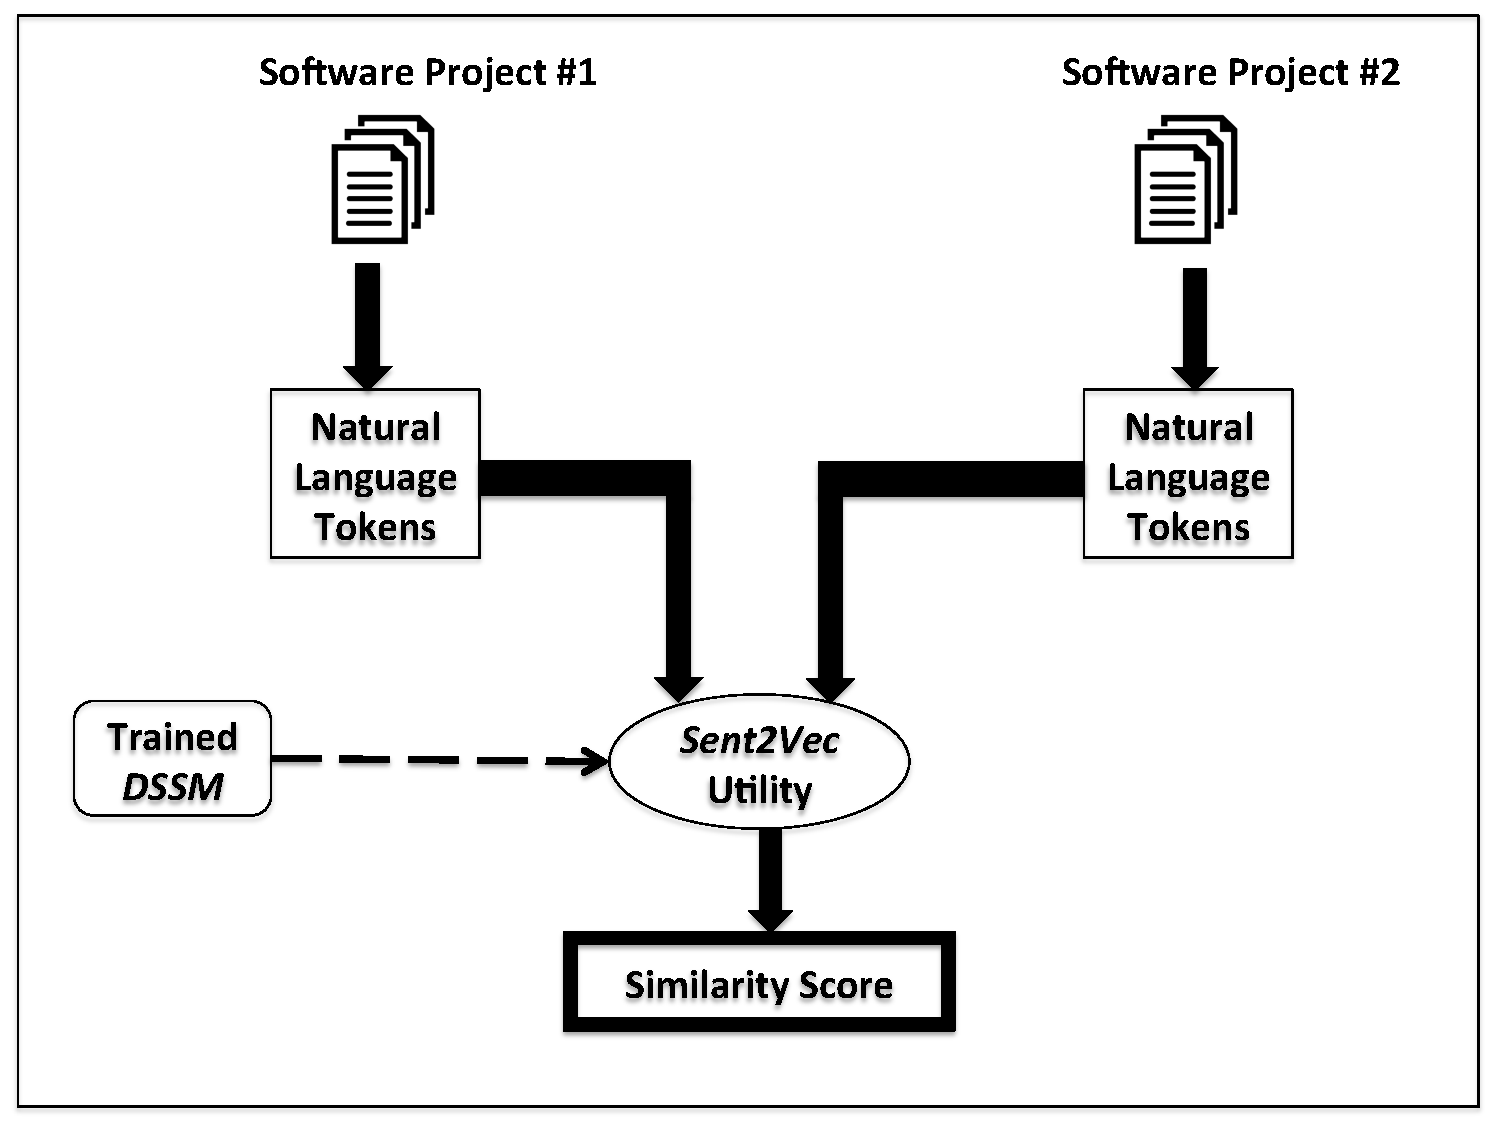
\includegraphics[scale=0.35]{plots/Diagram.pdf}
\caption{Major Steps Used in the Paper}
\label{fig-meth}
\end{figure}

\subsection{Collecting Software Repositories}
\label{proj_collect}
For analysis the author used popular Github projects written in three languages: C, C\#, and Java. The author hypothesizes that semantic similarity might be different for different projects in different programming languages, and analysis of such aspect can bring better insight with respect to semantic similarity. Keeping this assertion in mind, the author has considered three different programming languages: C, C\#, and Java. 

The author selected projects that were `trending' on Github between March 01, 2016 ~ March 30, 2016, and had a size in between 1MB ~ 100MB. The process was repeated for three programming languages namely C, C\#, and Java.  By implementing this process two projects from the C language, one project from the C\# language, and three projects from the Java language. Please note that `trending' is a feature of Github that ranks Github repositories that gained popularity amongst Github users for a certain time period such as a day, a week, or a month. 
\subsection{Token Extraction}
\label{token_extract}
The process of semantic similarity involves a collection of words or tokens using which a semantic model will be built to quantify the semantic similarity between two projects. To achieve this goal, 
the author used a two step process to gather necessary tokens from each of the software repositories of interest. These steps are presented below: 
\begin{itemize}
\item{The author used an open source tool called SrcML.NET to extract all the tokens from each repository. The SrcML.NET program takes the directory of each repository as input, and produces all tokens in one xml file.}
\item{The author used another open source tool called Swum.NET that filters the tokens generated from SrcML.NET. The motivation of executing this step was to obtain natural language tokens from the tokens generated in the previous step by conducting the pre-processing steps: 
\begin{itemize}
\item{convert camel-case and pascal-case tokens into natural language tokens}
\item{convert alpha-numeric tokens into natural language tokens such as converting to \textit{\_a\_variable} to \textit{a}, \textit{variable}}
\item{remove tokens that are a length of one }
\item{remove tokens from the token collection that are stop words in the English language}
\item{remove tokens from the token collection that are programming language specific keywords such as void, int, and main. }
\end{itemize}
}
\end{itemize}
After performing this step for each repository a .tsv file was created that was later used in training semantic models as well as evaluating the semantic similarity of software repositories. 
\subsection{Training Semantic Models}
\label{train_dssm}
The author has used the Deep Structured Semantic Model (DSSM) to quantify the semantic similarity between projects. According to Huang et al.~\cite{Huang:CIKM} DSSM learns from a query or a document which can be used to compute semantic similarity. DSSM trains itself by projecting semantically similar phrases that are close to other, and projecting semantically dissimilar phrases that are further to another. 
DSSM also provides configuration options to create different training models from the same document. Amongst these configuration options the author has used two parameters namely \textit{BATCHSIZE}, and \textit{MAX\_ITER}. \textit{BATCHSIZE} refers to how many training pairs can be used to train. \textit{MAX\_ITER} refers to the total count of iterations DSSM will use to create the training model.            
Similar to Yih et al.~\cite{wen:yih:semantic:parsing} the author performed the following actions to create the training model for each configuration: 
\begin{itemize}
\item{Shuffle the query pairs using the \textit{WordHash} utility with the \textit{shuffle} flag. }
\item{Following Gao et al.~\cite{gao:interesting:emnlp} the author generate the sequence of letter trigram features using the \textit{WordHash} utility with the \textit{pair2seqfea} flag. }
\item{The generated sequences of letter trigram features are converted to binary files using the \textit{WordHash} utility with the \textit{seqfea2bin} flag. }
\item{Next, the noise distribution of the training data is calculated using the \textit{ComputelogPD} utility.}
\item{Using a configuration file, and the \textit{DSSM\_Train} utility, the author created training models that are used to perform the analysis of this paper. The author describes which model is used for what experiment in Section~\ref{exp}.}
\end{itemize}

\subsection{Experiments}
\label{exp}
The author has designed four experiments to evaluate the similarity between two projects, in a pair-wise fashion. In these experiments the author has varied the training model with respect to DSSM configuration parameters as well as the documents that are using. Table~\ref{table-experiments} presents the experiments and the parameters that were changed. The experiments are referred by their names in Section~\ref{results}. 

In each of these experiments, similar to Huang et al.~\cite{Huang:CIKM}'s approach the author has used the Sent2Vec utility for comparing the six projects of interest. Sent2Vec uses cosine similarity to quantify the vectors of tokens amongst two projects~\cite{Huang:CIKM}. In each of the experiment, the six projects are compared in a pair-wise manner i.e. each of the six projects are compared to the rest of the five projects of interest. The author has followed the format of the provided example that comes with the Sent2Vec utility\footnote{http://research.microsoft.com/en-us/downloads/731572aa-98e4-4c50-b99d-ae3f0c9562b9/} to compare the similarity between two projects. The input files to the Sent2Vec utility was created in the following manner: the author splitted the natural languages tokens of the two projects of interest into 100000 buckets. Each line in the input file
corresponded to the tokens for both projects in each bucket. For example, line \#1 in the input file corresponded to the tokens in bucket\#1, for both projects. The process was repeated for each combination of projects, and as a result, 30 input files were created.
\begin{table}[]
\centering
\caption{Experiments Used in the Study}
\label{table-experiments}
\begin{tabular}{lll}
\hline
Name & Training Source & MAX\_ITER   \\
\hline 
Experiment-1 & Largest  repository &  500  \\
Experiment-2 & Largest  repository &  100,000  \\
Experiment-3 & Smallest repository &  500  \\
Experiment-4 & Smallest repository &  100,000  \\
\hline 
\end{tabular}
\end{table} 
The `Training Source' column in Table~\ref{table-experiments} corresponds to the repository of how the DSSM model will be trained. For example, in Experiemnt-1, and Experiemnt-3, the natural language tokens from the largest and the smallest repositories of the six software projects that are used in the study will train the DSSM model.    

Sent2Vec generates scores for each line in the input file. This score reflects the semantic similarity scores between the tokens that are separated by tabs. The author used a median approach to get the overall semantic score between two projects i.e. the median of all the scores for each line in the input file was used to determine the semantic similarity. For example, if the semantic similarity scores between project P and project Q is [0.1, 0.01, 0.54, 0.21, -0.43, 0.76, 0.31], then the semantic similarity is measured as 0.21, according to the author's proposed approach.  
      
 
%%%%%%%%%%%%%%%%%%%%%%%%%%%%%%%%%%%%%%%%%%%%%%%%%%%%%%%%%%%%%
%%%%%%%%%%%%%%%%%%%%% This is Results section %%%%%%%%%%%%
%%%%%%%%%%%%%%%%%%%%%%%%%%%%%%%%%%%%%%%%%%%%%%%%%%%%%%%%%%%%%
 

\section{Results}
\label{results}
The author describes relevant empirical findings in this section.   
\subsection{Software Repositories}
\label{res_proj_collect}
Table~\ref{table-repos} presents the repositories names and the number of tokens for each project after applying filtering techniques used in the study. 
\begin{table}[]
\centering
\caption{Repositories Used in the Study}
\label{table-repos}
\begin{tabular}{lllll}
\hline
Name &  Version or Branch & Language & Size (MB) & Count   \\
\hline
Git\footnote{https://github.com/git/git} & master & C & 6.60 & 247,303  \\
Redis\footnote{https://github.com/antirez/redis/tree/3.2} & 3.20 & C  & 1.70 & 183,295 \\
ShareX\footnote{https://github.com/ShareX/ShareX} & master & C\# &  6.40 & 788,962 \\
Douya\footnote{https://github.com/DreaminginCodeZH/Douya} & master & Java & 9.60  & 781,618 \\
RxJava\footnote{https://github.com/ReactiveX/RxJava/tree/master} & master & Java &  1.00 & 560,690 \\
SeeWeather\footnote{https://github.com/xcc3641/SeeWeather} & master & Java  &  3.20 & 164,263\\
\hline
\end{tabular}
\end{table}

Table~\ref{table-repos} presents the count of tokens achieved from each repository after performing the filtering steps. According to Table~\ref{table-repos} the largest and the smallest repositories used in the study are ShareX, and SeeWeather respectively. The filtered natural language tokens obtained from ShareX, and SeeWeather are used to create two different training models for DSSM. The goal of creating two different training models is to see if inclusion of tokens might have an impact of similarity measure. The scripts used to create the training DSSMs and used to execute Sent2Vec utility for Experiemnt-1, 2, 3, and 4 are available online~\footnote{http://tiny.cc/ymroay}. The files that are used as input to the Sent2Vec utility are available online~\footnote{https://github.com/akondrahman/Miscellaneous/tree/master/OpenSourceChallenge/input-to-sent2vec}. The output of the Sent2Vec utility for each of the input files are also available online~\footnote{https://github.com/akondrahman/Miscellaneous/tree/master/OpenSourceChallenge/output-of-sent2vec}. A sample snapshot of one of the input files to Sent2Vec and the corresponding output is provided in Figure~\ref{fig-sample-output}(a), and Figure~\ref{fig-sample-output}(b) respectively. As shown in in Figure~\ref{fig-sample-output}(a), the left column corresponds to the tokens of one project, whereas the tokens on the right column corresponds to the tokens of the other project, in a pair-wise comparison.       
  
\begin{figure}[htbp]
\centering
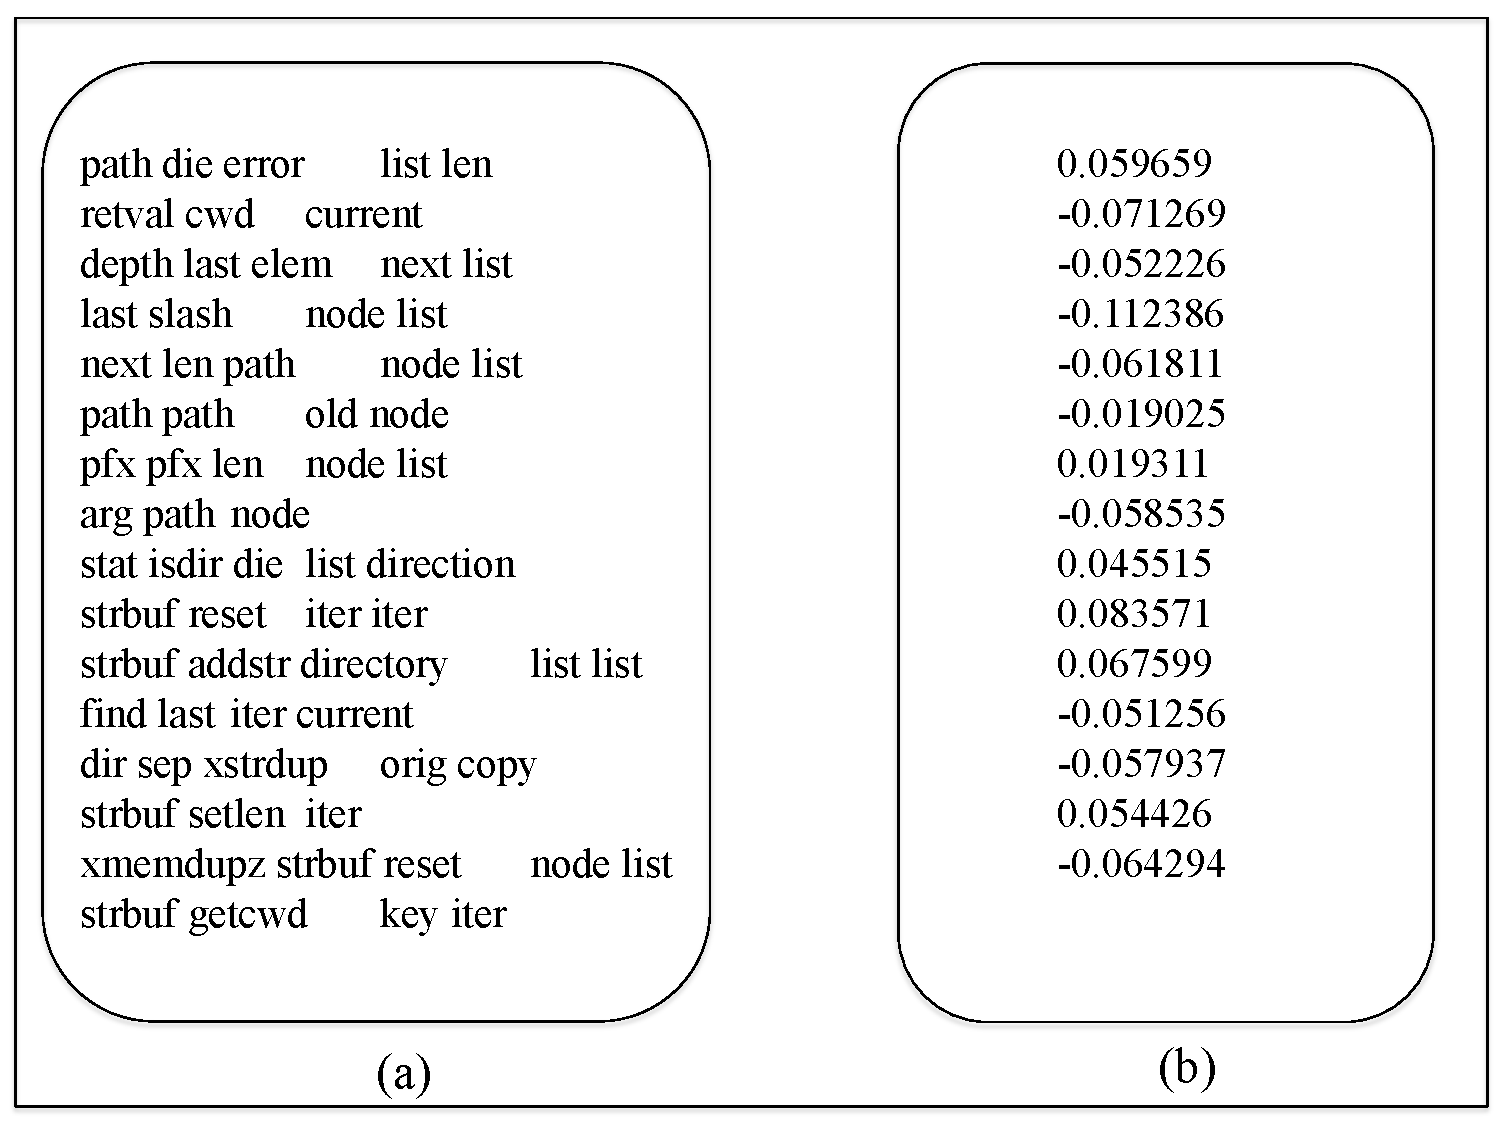
\includegraphics[scale=0.35]{plots/io_sent2vec.pdf}
\caption{Sample Input and Output Used for Sent2Vec}
\label{fig-sample-output}
\end{figure}
\subsection{Similarity}
\label{res_similarity}

As stated before in Section~\ref{meth} the author used two different training models as well as used different values for the two parameters of DSSM namely \textit{MAX\_ITER} and \textit{TARGET\_LAYER\_DIM}. The combination of these settings led to different experiments. 
% and the findings from each of these experiments are presented in Table~\ref{table-res-exp1}, ~\ref{table-res-exp2}, ~\ref{table-res-exp3}, and ~\ref{table-res-exp4} respectively for Expriment-1, 2, 3, and 4. 
\begin{table}[]
\centering
\caption{Results for Experiment-1}
\label{table-res-exp1}
\begin{tabular}{lllllll}
\hline
           & Git & Redis & ShareX & Douya & RxJava & SeeWeather \\
\hline
Git        & \bf{---} & 0.001 & 0.000 & 0.003 & 0.001 & 0.001 \\
Redis      & 0.000 & \bf{---} &  -0.001 &  -0.005 &  0.003 & -0.002 \\
ShareX     & 0.005 & 0.008 & \bf{---} & 0.011 & \bf{\textit{0.033}} & 0.003 \\
Douya      & 0.002 & 0.004 & -0.015 & \bf{---} &  -0.005 & 0.008  \\
RxJava     & 0.000  & 0.001 & -0.143 & -0.012 & \bf{---} & -0.003  \\     
SeeWeather & 0.001 & 0.000 & -0.011 & 0.000 & 0.000 & \bf{---} \\     
\hline
\end{tabular}
\end{table}

According to Table~\ref{table-res-exp1} the most similar projects are ShareX and RxJava as they have the highest semantic similarity scores. Interestingly, ShareX is written in C\#, and RxJava is written in Java. Please recall that the semantic similarity score is the median of all the semantic scores between the natural language tokens of the two corresponding software projects that are splitted across 100,000 buckets. Please note that the entries in Table~\ref{table-res-exp1} and~\ref{table-res-exp3} are not symmetric across the diagonal as the order of tokens in the input file for two projects can be different.  

\begin{table}[]
\centering
\caption{Results for Experiment-3}
\label{table-res-exp3}
\begin{tabular}{lllllll}
\hline
           & Git & Redis & ShareX & Douya & RxJava & SeeWeather \\
\hline
Git        & \bf{---} & 0.001 & 0.000 & -0.003 & 0.001 & -0.001 \\
Redis      & 0.000 & \bf{---} & -0.001 & -0.005 & 0.003 & -0.002 \\
ShareX     & 0.005 & 0.008 & \bf{---} & 0.011 & \bf{\textit{0.033}} & 0.003 \\
Douya      & 0.002 & 0.004 & -0.015 & \bf{---} & -0.005 & 0.008 \\
RxJava     & 0.000 & 0.001 & -0.014 & -0.012 & \bf{---} & -0.004 \\     
SeeWeather & 0.000 & 0.000 & -0.011 & 0.000 & 0.000 & \bf{---} \\     
\hline
\end{tabular}
\end{table}
From Table~\ref{table-res-exp3} the author observes that the similarity scores are overall the same between overall the projects. For further investigation the author has applied the following hypothesis test: 
\begin{itemize}
\item{$H_{0}$: The semantic similarity scores for Experiment-1 and Experiment-3 are not different. }
\item{$H_{A}$: The semantic similarity scores for Experiment-1 and Experiment-3 are different. }
\end{itemize} 
With 99\% statistical confidence the author has observed that the semantic similarity scores between Experiment-1 and Experiment-3 are not statistically different. Furthermore, the author has applied more hypothesis tests to observe if the semantic similarity scores obtained in each experiment is different to that of the others. The author has observed that there are no significant differences between the semantic similarity scores of Experiment-1, 2, 3, and 4. As the empirical findings of Experiment-2 and Experiment-4 are similar to that of Experiment-1 and Experiment-3, respectively, the author does not present findings for Experiment-2 and Experiment-4 in this paper. 
  
\textbf{Observations: } The author presents the following observations from the empirical findings of the study: 
\begin{itemize}
\item{ DSSM and Sent2Vec has the potential to capture semantic similarity between two software projects that are written in different programming languages. For example, the author has showed in this study that the highest similarity score in all experiments were between ShareX and RxJava. }
\item{Number of iterations to train DSSM did not have an impact on the semantic similarity between software projects as the semantic score obtained from all experiments are not significantly different. }
\item{The natural language tokens obtained from two different repositories did not have an impact on the semantic similarity score as the semantic score obtained from all experiments are not significantly different. }
\end{itemize}


%%%%%%%%%%%%%%%%%%%%%%%%%%%%%%%%%%%%%%%%%%%%%%%%%%%%%%%%%%%%%
%%%%%%%%%%%%%%%%%%%%% This is discussion section %%%%%%%%%%%%
%%%%%%%%%%%%%%%%%%%%%%%%%%%%%%%%%%%%%%%%%%%%%%%%%%%%%%%%%%%%%

\section{Discussion}
\label{discussion}
In this section the author discusses the implications of the empirical findings for programmers and researchers.  
\subsection{Identifying Re-usable Software Components}
Modern software teams have to maintain numerous software repositories. Software developers might have to use one or multiple components across one or different software repositories. Navigating through multiple software repositories to identify one or multiple components for re-use can be non-trivial as the process involves cognitive effort~\cite{parnin:MRI:brain:programming} and time~\cite{zimmerman:code:search}. An automated software tool that identifies similar software components within the software team, as well as in an open source software repository hub such as Github or Sourceforge\footnote{http://sourceforge.net/}, eventually saving software developers' time and effort.          
\subsection{Software Development in a Distributed Environment}
In many organizations software teams are geo-graphically distributed. For the purpose of software re-usability, coordinating amongst such distributed teams can be non-trivial as these teams might be in different time zones. An automated tool that captures semantic similarity across projects can be helpful in this regard. By-passing the communication and co-ordination methods such as setting up a Skype meeting, the tool can find and recommend software components that are similar to the developers' needs.   
\subsection{Application in Software Security}
Semantic similarity between two projects has the potential to be used to estimate software vulnerability and defects. For example, if component A of project X has vulnerabilities, and if component B of project Y is similar to that of component A, then component B might be susceptible to vulnerabilities. Such estimation can help software teams to apply a pro-active approach in preventing software vulnerabilities. For example, after developing a certain component C, a software team can investigate how similar it is to a known vulnerable software component. If the team finds strong similarity then that can be treated as an indication of component C being vulnerable. Such approach might reduce the probability of releasing vulnerable software components to end-users. 
\subsection{Intelligent IDE Design}  
Effective similarity measurement techniques between software projects can revolutionize code search features that are already existing in current desktop and cloud-based IDEs. Overall, current IDEs provide auto-completion features, as well as recommendations for tasks, and recommendations for code artifacts within the software project. Within an IT organization software teams can be geographically distributed, and can have large amount of software repositories. In such conditions semantic-based similarity approaches can help to narrow down the search space for IDEs to recommend the relevant software components. For example, when the developer types the word \textit{crypto}, the IDE might display the relevant package that has the implementation of cryptographic methods located in a remote repository. The IDE can also display multiple components based on a suitable ranking measure.  




\section{Limitations}
\label{limitation}
We discuss the limitations of our study in this section as follwowing: 

\textbf{Lack of Ground Truth:} In Section~\ref{results} the author has showed how DSSM and Sent2Vec can be used to compute similarity scores between different software projects without describing the ground truth. The author has not demonstrated why or how RxJava and ShareX have the highest simialrity scores.   

\textbf{Granularity:} The tokens for each of the nine software projects are calculated at a file level. The author has not discussed how tokens collected at other granularities such as namespaces, binaries, or classes might have a different impact on the similarity scores between projects. 

\textbf{Selection of Software Repositories:} The author has selected a small set of repositories for illustration of the methodology. The size of these software repositories varied between 1 MB~100 MB. Further investigation is required to appropriately assess the capability of DSSM and Sent2Vec to quantify semantic similarity between software projects. 

\textbf{Use of Parameters:} As shown in Section~\ref{related} and Section~\ref{meth} the author has selected and used a specific set of parameters for training the DSSM models. Further exploration and experimentation with all parameters of DSSM is needed to fully assess DSSM's capability of discovering semantic similarity between software projects.       
 

\section{Challenges}
\label{challenges}
Conducting necessary experiments using DSSM was challenging in the following ways: 

\begin{itemize}
\item{\textbf{Resolving CudaLib Dependency}: DSSM relies on the \textit{CudaLib} dll to perform its computations. Unfortunately, the provided executable binary file, hosted on the website\footnote{http://research.microsoft.com/en-us/projects/dssm/} did not have that added that dependency. As a result, the author was getting a ``DllNotFoundException'' when creating different DSSM training models for Experiment - 1, 2, 3, and 4. To resolve this, the author first investigated the source code of DSSM, and having observed DSSM's dll dependency on CudaLib, installed \textit{CUDA Toolkit 7.5} and re-executed the Visual Studio project for CudaLib, and DSSM. With the newly created binary the author conducted the necessary experiments.  }

\item{\textbf{Format of Input for DSSM and Sent2Vec}: Understanding the format of what is passed into DSSM and Sent2Vec was non-trivial. The author explored the contents of the raw .tsv as well as the `pairs.txt' files to understand the formatting for input files.}
\end{itemize}  

\section{Conclusion}
\label{conclusion}
 
In this paper the author has described how Microsoft's Deep Semantic Similarity Model (DSSM) and Sent2Vec can be used to identify and quantify semantic similarity between software projects. The author has also discussed the future implications of this study and how future research in this area can help software teams to identify re-usable software components with reduced effort. The author believes future academic and industry research in this area has the possibility of revolutionizing standard organizational efforts in software engineering.   





\bibliographystyle{IEEEtran}
\bibliography{bibs/opensource.bib}









% that's all folks
\end{document}


